%%%%%%%%%%%%%%%%%%%%%%%%%%%%%%%%%%%%%%%%%%%%%%%%%%%%%%%%%%%%%%%%%%%%%%%%%%%%%%%%
%2345678901234567890123456789012345678901234567890123456789012345678901234567890
%        1         2         3         4         5         6         7         8

%\documentclass[letterpaper, 10 pt, conference]{ieeeconf}  % Comment this line out if you need a4paper

\documentclass[a4paper, 10pt, conference]{ieeeconf}      % Use this line for a4 paper

\IEEEoverridecommandlockouts                              % This command is only needed if
                                                          % you want to use the \thanks command

\overrideIEEEmargins                                      % Needed to meet printer requirements.

% See the \addtolength command later in the file to balance the column lengths
% on the last page of the document

% The following packages can be found on http:\\www.ctan.org
%\usepackage{graphics} % for pdf, bitmapped graphics files
%\usepackage{epsfig} % for postscript graphics files
%\usepackage{mathptmx} % assumes new font selection scheme installed
%\usepackage{times} % assumes new font selection scheme installed
%\usepackage{amsmath} % assumes amsmath package installed
%\usepackage{amssymb}  % assumes amsmath package installed
\usepackage[backend=biber]{biblatex}
\bibliography{Report}


\title{\LARGE \bf
Event handling using static and dynamic task allocation strategies
}


\author{Brice Platerrier, Martin Vassor and Arnaud Wald}

\begin{document}

\maketitle
\thispagestyle{empty}
\pagestyle{empty}

%%%%%%%%%%%%%%%%%%%%%%%%%%%%%%%%%%%%%%%%%%%%%%%%%%%%%%%%%%%%%%%%%%%%%%%%%%%%%%%%
\begin{abstract}

TO BE COMPLETED

\end{abstract}

%%%%%%%%%%%%%%%%%%%%%%%%%%%%%%%%%%%%%%%%%%%%%%%%%%%%%%%%%%%%%%%%%%%%%%%%%%%%%%%%
\chapter*{Introduction}
This project deals with task allocation where there are multiple types of tasks. The robots will handle tasks that appear throughout the environment according to threshold-based task allocation strategies.

We first propose static strategies where the weights of the stimuli are fixed and the thresholds are individual. We compare the homogeneous experiment, where all robots have the same threshold, to the heterogeneous case, where the robots adapt there thresholds depending on the time spent in search or by specializing in a peculiar task.

In an attempt to improve performance by avoiding multiple robots selecting the same task, we analyze the benefits of a dynamic strategy where each robot emits a virtual potential field for the task type it selected. The robots use the intensities of the potential field separately for each type of task and use this additional information to dynamically adjust the weights of the stimuli.

% All strategies were implemented and tested in Webots. Since the dynamic strategy has a number of parameters that can be optimized, we ran particle swarm optimization.


\section{Experiments}
To assess the efficiency of our algorithms, we consider the task handling problem where 3 types of tasks appear in a closed arena. A task, represented as a colored cylinder (with colors being red, green or blue), is processed by a robot being in its vicinity for a given amount of time, but is not processed faster as the number of robots close to its position increases. Once a task is processed, it disappears and a new one appears at a random location. The goal of our algorithms is to optimize the task allocation so as to prevent multiple robots from picking the same task.

Robots identify the tasks with the on-board camera. Each robot evaluates stimuli for red, green and blue tasks based on its local camera observations. Each robot analyzes the row of pixels in the middle of its camera image, then computes the sizes of the biggest clusters of each color. The initial stimuli for red, green and blue are those sizes in pixel, but they can be modulated to allow a better repartition of robots among tasks. The  robot  will  then select the  task according to our threshold-based algorithms.

In order to emit the virtual potential field, the robots are endowed with radio emitters (and receivers) that broadcasts (and gathers) the relevant information perceived by the robots, within a short range. These information are then fed into our public and individual threshold-based algorithm to dynamically adapt the stimuli.

\textbf{Implementation:}
The framework used during the course of the project allowed us to test 3 main approaches. They could be divided in two categories, one being private (static case) and the other being public (dynamic case). In the first case, we considered both homogenous (fixed and identical thresholds among robots) and heterogeneous (adaptive thresholds based on each robot's vision or time spent in search mode) cases. In the second case, we took advantage of the local potential field emissions perceived by the robots to adjust the weights of each color stimulus to improve task allocation and tried both fixed and variable thresholds.
Simulations were run on the realistic robot simulator WeBots. The agents used are e-pucks robots. The arena configuration can be seen on figure \ref{screenshot}.

\begin{figure}[thpb]
	\begin{center}
		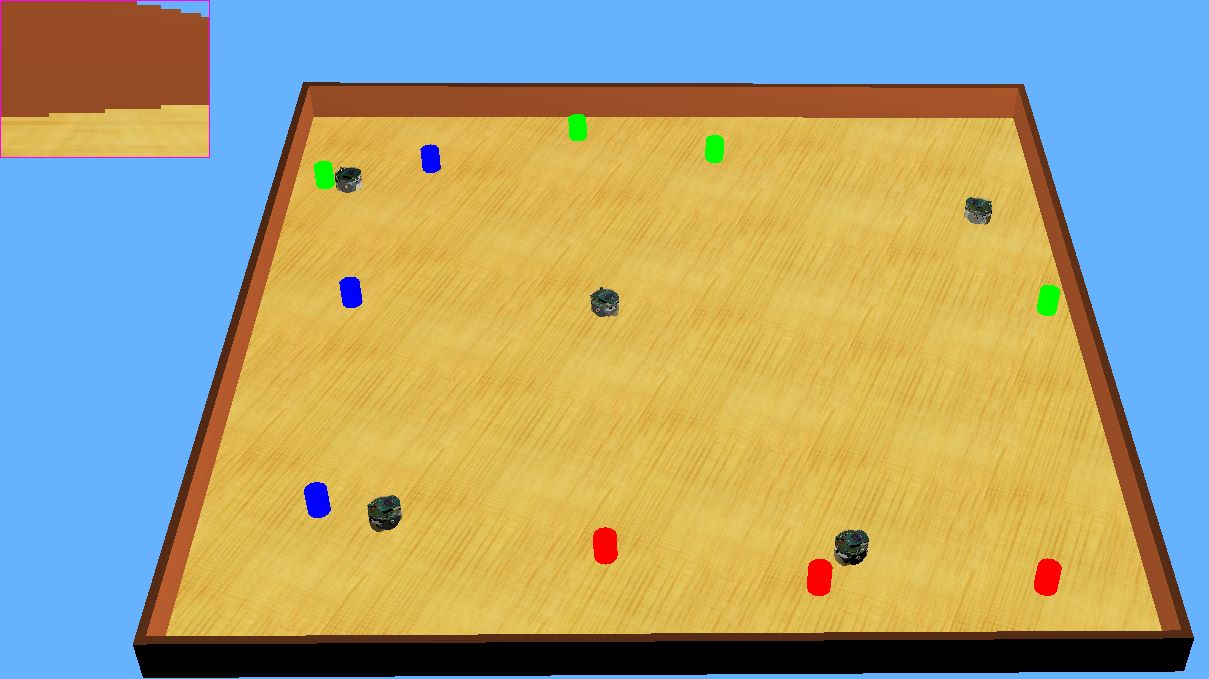
\includegraphics[width=8.5cm]{Pictures/Capture.png}
		\caption{The disposition of the arena with the e-puck robots (in gray/dark green) and the different tasks represented by red, green and blue cylinders. On the top-left corner is displayed the camera image of one of the robots.}
    \label{screenshot}
	\end{center}

\end{figure}

\textbf{Task Allocation Mechanism:}
For the simulations to be comparable, we used the same Finite State Machine (FSM) for all simulations and all types of algorithms. This FSM is described in Figure \ref{fsm}. The behavior of the robots could be described as follows. All the robots are initialized in the first state ($S1$) that consists in spinning around and processing the image from the camera to determine if task needs to be handled. Once a task is picked, the robot changes state and goes directly towards the task ($S2$). To avoid collisions between robots, obstacle avoidance is added is this state. If the robot happens to lose track of its target (when the stimulus gets lower than a given threshold), it switches back to $S1$. When the robot is close enough to the task, it slows down for a given amount of time to process the task ($S3$). Once the task is processed, the robot will go back in $S1$.

\begin{figure}[thpb]
	\begin{center}
		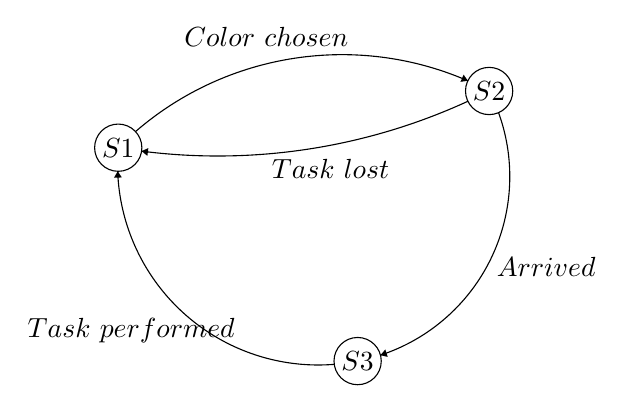
\begin{tikzpicture}[scale=0.1]
			\tikzstyle{every node}+=[inner sep=0pt]
			\draw [black] (18.1,-22.4) circle (3);
			\draw (18.1,-22.4) node {$S1$};
			\draw [black] (65.2,-15.2) circle (3);
			\draw (65.2,-15.2) node {$S2$};
			\draw [black] (48.5,-49.5) circle (3);
			\draw (48.5,-49.5) node {$S3$};
			\draw [black] (66.396,-17.949) arc (19.90503:-71.82612:23.863);
			\fill [black] (51.4,-48.75) -- (52.32,-48.97) -- (52.01,-48.02);
			\draw (66.12,-37.6) node [right] {$Arrived$};
			\draw [black] (45.53,-49.914) arc (-85.42932:-178.00132:25.487);
			\fill [black] (18.03,-25.4) -- (17.56,-26.21) -- (18.56,-26.18);
			\draw (19.74,-44.02) node [below] {$Task\mbox{ }performed$};
			\draw [black] (20.293,-20.354) arc (130.86729:66.51532:40.086);
			\fill [black] (62.5,-13.9) -- (61.96,-13.13) -- (61.56,-14.04);
			\draw (36.9,-9.67) node [above] {$Color\mbox{ }chosen$};
			\draw [black] (62.5,-16.506) arc (-65.31733:-97.30006:76.07);
			\fill [black] (21.07,-22.84) -- (21.8,-23.44) -- (21.92,-22.45);
			\draw (45.05,-23.77) node [below] {$Task\mbox{ }lost$};
		\end{tikzpicture}
		\caption{The Finite-State-Machine of the robots}
    \label{fsm}
	\end{center}

\end{figure}

\subsection{Private, Fixed Threshold-based Algorithm}
In this first experiment, the same response threshold is assigned to each robot and identical for each color (no specialization). Various agent behaviors are obtained thanks to the local perception of the environment and the private assessment of the demand. We considered both the deterministic and probabilistic task allocation. In the latter, the robots where using a sigmoid function to determine if a given task should be processed or not.

\subsection{Private, Adaptive Threshold-based Algorithm}
The next case considers adaptive thresholds to improve the robustness of the task allocation strategy. As the number of robots is not equal nor a multiple of the number of task categories, we chose to consider two adaptation methods. The first one considers the robots to be "colorblind", the threshold is the same for each color and the adaptation consists in lowering the value of all the thresholds as the robots remain in search mode (and conversely, increasing the value if a task is performed). The second one proceeds to a specialization of the robots as they perform a given type of task repeatedly. This approach can be combined with the previous one by lowering the thresholds of the robots if too much time is spent in search mode.

\subsection{Public, Fixed \& Variable Threshold-based Algorithm}
The final approach adds communication between the robots to share information about the tasks identified through vision. The method consists in using the information received through radio communication to change the weights of the color stimuli so as to avoid selecting the same task as another robot.

In order to neglect the influence of neighbors being too far from a robot position, we chose to limit the maximum range at which the emissions were perceived. The value was set so that the corresponding area of reception of a given robot was one fifth of the total area of the arena. Thus, each robot was more inclined to work in its own area and could deal with neighbors entering the area and likely to choose the same task. Furthermore, we chose to modify the saturate the signal strength of the received emissions. Indeed, for the robot to react sufficiently fast if it picked the same task as its neighbor, the signal strength had to be limited to a maximum value before normalization of the received perceptions. This assumption somehow goes beyond the initial idea of potential field but is perfectly workable using radio communications. It should also be noted that the model adopted here could be applicable to really noisy and imprecise receiver.

The sent information had to be meaningful for the robots to assess the situation correctly. Although we tried to send the proximity of the closest task for each color, we eventually restrained the information sent to the closeness of the chosen task. This information was then updated and sent as long as the robot was traveling to the task. Based on this information, the robots could decide to search for a new task if the same color was chosen by a neighbor that was closer to the task.

In this project, we propose a function to update each color stimulus based on the information perceived by the neighbors. This function is comprised of two factors: the weight of local stimuli, $\alpha$, and the weight of neighbors stimuli, $\beta$. The first factor reduces the power of the stimuli as the received values increases. The second one allows the robot to still have a chance to perform the task it had chosen if it is closer to it than its neighbors. If the decrease in the stimulus is high enough (i.e. the stimulus is less than a given threshold, called "lost threshold"), the robot will abandon the task it had chosen and resume search. The update of the stimulus for color $i$ is done as follows:

$$
\sigma_{new}(i) = \sigma_{prev}(i)*(1 + \beta) - \alpha*R(i) \eqno{(1)}
$$

where $\sigma_{new}$ and $\sigma_{prev}$ are the new and previous stimulus values and $R(i)$ is the normalized reception of color $i$.


\chapter{Results \& Discussion}
[EXPERIMENT 1: WE COULD TRY DIFFERENT THRESHOLD VALUES AND COMPARE PERFORMANCES | EXPERIMENT 2: WE COULD TRY DIFFERENT ADAPTATION MECHANISM (VISION OR TIME IN SEARCH MODE = COLORBLIND) AND COMPARE RESULTS | EXPERIMENT 3: WE COULD TRY DIFFERENT ADAPTATION FUNCTION FOR STIMULI AND COMPARE RESULTS | LAST PART: COMPARE ALL ALGORITHMS WITH BEST PERFORMANCE]

\section{Conclusion}


%\addtolength{\textheight}{-12cm}   % This command serves to balance the column lengths
                                  % on the last page of the document manually. It shortens
                                  % the textheight of the last page by a suitable amount.
                                  % This command does not take effect until the next page
                                  % so it should come on the page before the last. Make
                                  % sure that you do not shorten the textheight too much.


\printbibliography

\end{document}
